%----------------------------------------------------------------------------------------
%    PACKAGES AND THEMES
%----------------------------------------------------------------------------------------
\documentclass[aspectratio=169,xcolor=dvipsnames]{beamer}
\makeatletter
\def\input@path{{../BeamerTemplate/theme/}}
\makeatother
\usetheme{CleanEasy}
\usepackage[utf8]{inputenc}
\usepackage{lmodern}
\usepackage[T1]{fontenc}
\usepackage{fix-cm}
\usepackage{amsmath}
\usepackage{mathtools}
\usepackage{listings}
\usepackage{xcolor}
\usepackage{hyperref}
\usepackage{graphicx}
\usepackage{booktabs}
\usepackage{tikz}
\usetikzlibrary{positioning, shapes, arrows, calc, decorations.pathreplacing, arrows.meta, backgrounds, patterns, overlay-beamer-styles}
\usepackage{etoolbox}

%----------------------------------------------------------------------------------------
%    LAYOUT CONFIGURATION
%----------------------------------------------------------------------------------------
\input{../BeamerTemplate/configs/configs}

%----------------------------------------------------------------------------------------
%    TITLE PAGE CONFIGURATION
%----------------------------------------------------------------------------------------
\title{Practical Applications \& Projects}
\subtitle{Building Real-World Systems with Data Structures}
\author{Minseok Jeon}
\institute{DGIST}
\date{\today}

\begin{document}

\begin{frame}
  \titlepage
\end{frame}

\begin{frame}{Outline}
  \tableofcontents
\end{frame}

% Introduction
\section{Introduction}

\begin{frame}{Course Overview}
  \begin{block}{Learning by Building}
    Apply data structures concepts by implementing complete, working systems
  \end{block}

  \vspace{0.3cm}
  \textbf{Projects Covered:}
  \begin{itemize}
    \item Text editor with undo/redo (Stack)
    \item Simple database index (B-Trees)
    \item Social network graph analysis (Graphs)
    \item Autocomplete engine (Tries)
    \item Memory allocator simulator (Free lists)
    \item Project structuring and testing
  \end{itemize}
\end{frame}

\begin{frame}{Why Practical Projects?}
  \textbf{Benefits:}
  \begin{itemize}
    \item \textbf{Deeper Understanding}: See how data structures solve real problems
    \item \textbf{Design Skills}: Learn to choose appropriate structures
    \item \textbf{Integration}: Combine multiple data structures effectively
    \item \textbf{Testing}: Develop comprehensive testing strategies
    \item \textbf{Portfolio}: Build projects for interviews and resumes
  \end{itemize}

  \vspace{0.3cm}
  \begin{alertblock}{Key Principle}
    Every project demonstrates a core data structure in a practical context
  \end{alertblock}
\end{frame}

% Text Editor with Undo/Redo
\section{Text Editor with Undo/Redo}

\begin{frame}{Project 1: Text Editor with Undo/Redo}
  \begin{columns}
    \begin{column}{0.5\textwidth}
      \textbf{Project Requirements:}
      \begin{itemize}
        \item Basic text operations: insert, delete, replace
        \item Undo last operation
        \item Redo previously undone operation
        \item Multiple undo/redo levels
        \item Clear redo stack on new operations
      \end{itemize}
    \end{column}

    \begin{column}{0.5\textwidth}
      \textbf{Core Data Structure:}
      \begin{itemize}
        \item \textbf{Stack} for undo/redo
        \item Two stacks: undo stack and redo stack
        \item Command pattern for operations
      \end{itemize}

      \vspace{0.3cm}
      \textbf{Complexity:}
      \begin{itemize}
        \item Undo/Redo: $O(1)$
        \item Operations: $O(n)$ worst case
      \end{itemize}
    \end{column}
  \end{columns}
\end{frame}

\begin{frame}{Design: Command Pattern}
  \begin{center}
    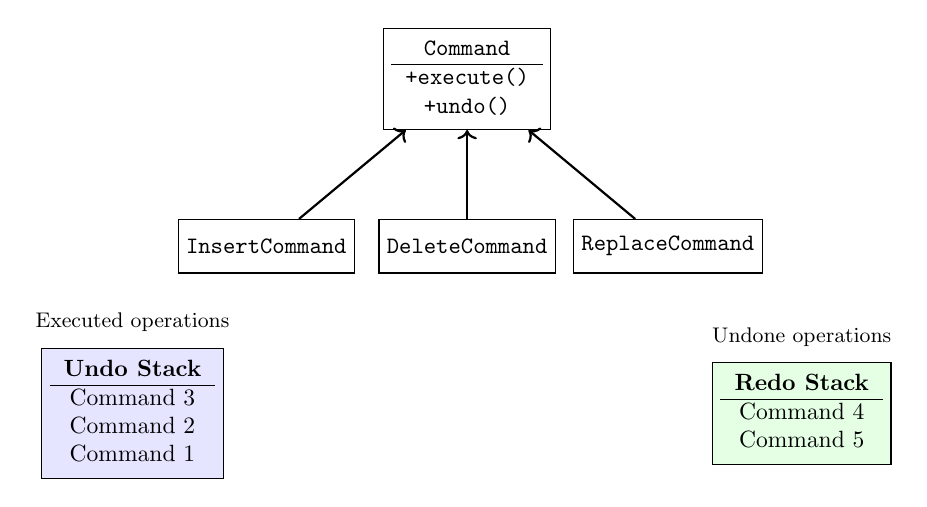
\begin{tikzpicture}[scale=0.85, every node/.style={scale=0.85}]
      % Command interface
      \node[draw, rectangle, minimum width=2.5cm, minimum height=1cm] (cmd) at (0, 0) {
        \begin{tabular}{c}
          \texttt{Command} \\
          \hline
          \texttt{+execute()} \\
          \texttt{+undo()}
        \end{tabular}
      };

      % Concrete commands
      \node[draw, rectangle, minimum width=2cm, minimum height=0.8cm] (insert) at (-3, -2.5) {
        \texttt{InsertCommand}
      };

      \node[draw, rectangle, minimum width=2cm, minimum height=0.8cm] (delete) at (0, -2.5) {
        \texttt{DeleteCommand}
      };

      \node[draw, rectangle, minimum width=2cm, minimum height=0.8cm] (replace) at (3, -2.5) {
        \texttt{ReplaceCommand}
      };

      % Arrows
      \draw[->, thick] (insert) -- (cmd);
      \draw[->, thick] (delete) -- (cmd);
      \draw[->, thick] (replace) -- (cmd);

      % Stacks
      \node[draw, rectangle, minimum width=2cm, minimum height=1.5cm, fill=blue!10] (undo) at (-5, -5) {
        \begin{tabular}{c}
          \textbf{Undo Stack} \\
          \hline
          Command 3 \\
          Command 2 \\
          Command 1
        \end{tabular}
      };

      \node[draw, rectangle, minimum width=2cm, minimum height=1.5cm, fill=green!10] (redo) at (5, -5) {
        \begin{tabular}{c}
          \textbf{Redo Stack} \\
          \hline
          Command 4 \\
          Command 5
        \end{tabular}
      };

      % Labels
      \node[above=0.1cm of undo] {\small Executed operations};
      \node[above=0.1cm of redo] {\small Undone operations};
    \end{tikzpicture}
  \end{center}
\end{frame}

\begin{frame}[fragile]{Implementation: Command Interface}
\begin{lstlisting}[language=Python, basicstyle=\tiny\ttfamily]
from abc import ABC, abstractmethod

class Command(ABC):
    """Abstract base class for text editor commands."""

    @abstractmethod
    def execute(self, text: List[str]) -> None:
        """Execute the command."""
        pass

    @abstractmethod
    def undo(self, text: List[str]) -> None:
        """Undo the command."""
        pass

class InsertCommand(Command):
    def __init__(self, position: int, text: str):
        self.position = position
        self.text = text

    def execute(self, text: List[str]) -> None:
        for i, char in enumerate(self.text):
            text.insert(self.position + i, char)

    def undo(self, text: List[str]) -> None:
        for _ in range(len(self.text)):
            text.pop(self.position)
\end{lstlisting}
\end{frame}

\begin{frame}[fragile]{Implementation: TextEditor Class}
\begin{lstlisting}[language=Python, basicstyle=\tiny\ttfamily]
class TextEditor:
    def __init__(self):
        self.text: List[str] = []
        self.undo_stack: List[Command] = []
        self.redo_stack: List[Command] = []

    def execute(self, command: Command) -> None:
        command.execute(self.text)
        self.undo_stack.append(command)
        self.redo_stack.clear()  # Clear redo on new operation

    def undo(self) -> bool:
        if not self.undo_stack:
            return False
        command = self.undo_stack.pop()
        command.undo(self.text)
        self.redo_stack.append(command)
        return True

    def redo(self) -> bool:
        if not self.redo_stack:
            return False
        command = self.redo_stack.pop()
        command.execute(self.text)
        self.undo_stack.append(command)
        return True
\end{lstlisting}
\end{frame}

\begin{frame}{Text Editor: Key Design Decisions}
  \begin{columns}
    \begin{column}{0.5\textwidth}
      \textbf{Stack Operations:}
      \begin{itemize}
        \item Push to undo stack on execute
        \item Pop from undo, push to redo on undo
        \item Pop from redo, push to undo on redo
        \item Clear redo stack on new operation
      \end{itemize}
    \end{column}

    \begin{column}{0.5\textwidth}
      \textbf{Extensions:}
      \begin{itemize}
        \item Compound commands (macro recording)
        \item History size limit
        \item Save state detection
        \item Text statistics
        \item Find and replace all
      \end{itemize}
    \end{column}
  \end{columns}

  \vspace{0.3cm}
  \begin{block}{Testing Strategy}
    \begin{itemize}
      \item Test each command type independently
      \item Test undo/redo sequences
      \item Test redo clearing on new operation
      \item Test edge cases (empty stack, invalid positions)
    \end{itemize}
  \end{block}
\end{frame}

% Database Index with B-Trees
\section{Database Index with B-Trees}

\begin{frame}{Project 2: Database Index using B-Trees}
  \begin{columns}
    \begin{column}{0.5\textwidth}
      \textbf{Project Requirements:}
      \begin{itemize}
        \item Store key-value pairs with sorted keys
        \item Insert, search, delete operations
        \item Handle large datasets efficiently
        \item Maintain balance automatically
        \item Support range queries
      \end{itemize}
    \end{column}

    \begin{column}{0.5\textwidth}
      \textbf{Core Data Structure:}
      \begin{itemize}
        \item \textbf{B-Tree} (order $t$)
        \item Each node: $t-1$ to $2t-1$ keys
        \item Self-balancing
        \item Disk-friendly (minimize I/O)
      \end{itemize}

      \vspace{0.3cm}
      \textbf{Complexity:}
      \begin{itemize}
        \item Search: $O(\log n)$
        \item Insert: $O(\log n)$
        \item Delete: $O(\log n)$
      \end{itemize}
    \end{column}
  \end{columns}
\end{frame}

\begin{frame}{B-Tree Structure}
  \begin{center}
    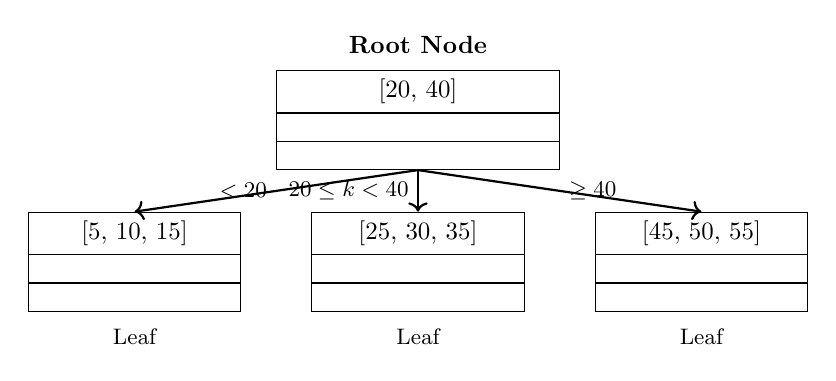
\begin{tikzpicture}[scale=0.9, every node/.style={scale=0.9}]
      % Root node
      \node[draw, rectangle split, rectangle split parts=3, minimum width=4cm] (root) at (0, 0) {
        \nodepart{one} [20, 40]
        \nodepart{two}
        \nodepart{three}
      };

      % Left child
      \node[draw, rectangle split, rectangle split parts=3, minimum width=3cm] (left) at (-4, -2) {
        \nodepart{one} [5, 10, 15]
        \nodepart{two}
        \nodepart{three}
      };

      % Middle child
      \node[draw, rectangle split, rectangle split parts=3, minimum width=3cm] (mid) at (0, -2) {
        \nodepart{one} [25, 30, 35]
        \nodepart{two}
        \nodepart{three}
      };

      % Right child
      \node[draw, rectangle split, rectangle split parts=3, minimum width=3cm] (right) at (4, -2) {
        \nodepart{one} [45, 50, 55]
        \nodepart{two}
        \nodepart{three}
      };

      % Arrows
      \draw[->, thick] (root.south) -- (left.north) node[midway, left, font=\small] {$< 20$};
      \draw[->, thick] (root.south) -- (mid.north) node[midway, left, font=\small] {$20 \le k < 40$};
      \draw[->, thick] (root.south) -- (right.north) node[midway, right, font=\small] {$\ge 40$};

      % Labels
      \node[above=0.1cm of root] {\textbf{Root Node}};
      \node[below=0.1cm of left] {\small Leaf};
      \node[below=0.1cm of mid] {\small Leaf};
      \node[below=0.1cm of right] {\small Leaf};
    \end{tikzpicture}
  \end{center}

  \vspace{0.3cm}
  \begin{block}{B-Tree Properties (order $t=3$)}
    \begin{itemize}
      \item Each node has $2 \le \text{keys} \le 5$ (except root)
      \item Keys are sorted within each node
      \item All leaves at the same level
    \end{itemize}
  \end{block}
\end{frame}

\begin{frame}[fragile]{Implementation: B-Tree Node}
\begin{lstlisting}[language=Python, basicstyle=\tiny\ttfamily]
class BTreeNode:
    def __init__(self, leaf=True):
        self.keys = []          # List of keys
        self.values = []        # List of values (for leaf nodes)
        self.children = []      # List of child nodes
        self.leaf = leaf        # Is this a leaf node?

class BTree:
    def __init__(self, t=3):
        """Initialize B-Tree with minimum degree t."""
        self.root = BTreeNode()
        self.t = t  # Each node: t-1 to 2t-1 keys

    def search(self, key, node=None):
        """Search for a key in O(log n) time."""
        if node is None:
            node = self.root

        i = 0
        while i < len(node.keys) and key > node.keys[i]:
            i += 1

        if i < len(node.keys) and key == node.keys[i]:
            return node.values[i] if node.leaf else self.search(key, node.children[i])

        return None if node.leaf else self.search(key, node.children[i])
\end{lstlisting}
\end{frame}

\begin{frame}[fragile]{Implementation: B-Tree Insert}
\begin{lstlisting}[language=Python, basicstyle=\tiny\ttfamily]
def insert(self, key, value):
    root = self.root

    # If root is full, split it
    if len(root.keys) == (2 * self.t) - 1:
        new_root = BTreeNode(leaf=False)
        new_root.children.append(self.root)
        self._split_child(new_root, 0)
        self.root = new_root

    self._insert_non_full(self.root, key, value)

def _split_child(self, parent, index):
    """Split a full child node."""
    t = self.t
    full_child = parent.children[index]
    new_child = BTreeNode(leaf=full_child.leaf)

    mid_index = t - 1
    # Move middle key up to parent
    parent.keys.insert(index, full_child.keys[mid_index])

    # Split keys and values
    new_child.keys = full_child.keys[mid_index + 1:]
    full_child.keys = full_child.keys[:mid_index]
    # ... (similar for values and children)

    parent.children.insert(index + 1, new_child)
\end{lstlisting}
\end{frame}

\begin{frame}{B-Tree Operations: Visual Example}
  \begin{center}
    \textbf{Inserting 17 into a full node causes split:}

    \vspace{0.3cm}
    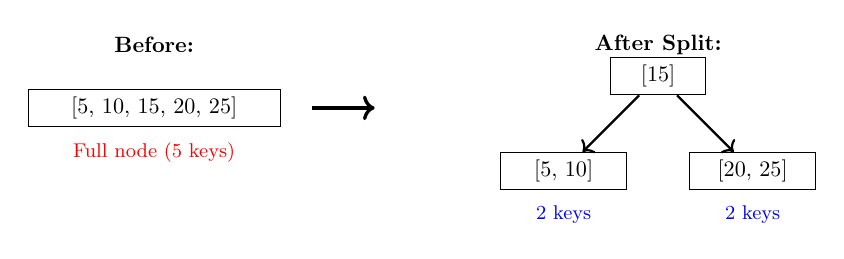
\begin{tikzpicture}[scale=0.8, every node/.style={scale=0.8}]
      % Before
      \node at (-5, 1) {\textbf{Before:}};
      \node[draw, rectangle, minimum width=4cm] (before) at (-5, 0) {
        [5, 10, 15, 20, 25]
      };
      \node[below=0.1cm of before, font=\small, red] {Full node (5 keys)};

      % Arrow
      \draw[->, very thick] (-2.5, 0) -- (-1.5, 0);

      % After
      \node at (3, 1) {\textbf{After Split:}};

      % Parent with middle key
      \node[draw, rectangle, minimum width=1.5cm] (parent) at (3, 0.5) {[15]};

      % Left child
      \node[draw, rectangle, minimum width=2cm] (left) at (1.5, -1) {[5, 10]};

      % Right child
      \node[draw, rectangle, minimum width=2cm] (right) at (4.5, -1) {[20, 25]};

      % Arrows
      \draw[->, thick] (parent) -- (left);
      \draw[->, thick] (parent) -- (right);

      \node[below=0.1cm of left, font=\small, blue] {2 keys};
      \node[below=0.1cm of right, font=\small, blue] {2 keys};
    \end{tikzpicture}
  \end{center}

  \vspace{0.3cm}
  \begin{itemize}
    \item Middle key (15) promoted to parent
    \item Left child contains smaller keys
    \item Right child contains larger keys
    \item Both children have valid number of keys
  \end{itemize}
\end{frame}

\begin{frame}{Database Integration}
  \begin{columns}
    \begin{column}{0.5\textwidth}
      \textbf{Simple Database System:}
      \begin{itemize}
        \item Primary key index (B-Tree)
        \item Secondary indexes (multiple B-Trees)
        \item Insert records with auto-increment ID
        \item Search by ID or indexed field
        \item Range queries
        \item Delete records
      \end{itemize}
    \end{column}

    \begin{column}{0.5\textwidth}
      \textbf{Use Cases:}
      \begin{itemize}
        \item Database management systems
        \item File systems (e.g., ext4, NTFS)
        \item Any sorted data on disk
      \end{itemize}

      \vspace{0.3cm}
      \textbf{Why B-Trees?}
      \begin{itemize}
        \item Minimize disk I/O
        \item Nodes = disk blocks
        \item Shallow tree (high branching factor)
        \item All leaves at same level
      \end{itemize}
    \end{column}
  \end{columns}
\end{frame}

% Social Network Graph Analysis
\section{Social Network Graph Analysis}

\begin{frame}{Project 3: Social Network Graph Analysis}
  \begin{columns}
    \begin{column}{0.5\textwidth}
      \textbf{Project Requirements:}
      \begin{itemize}
        \item Represent users and friendships
        \item Find degrees of separation (shortest path)
        \item Suggest friends (mutual connections)
        \item Detect communities
        \item Calculate influence metrics
        \item Clustering coefficient
      \end{itemize}
    \end{column}

    \begin{column}{0.5\textwidth}
      \textbf{Core Data Structure:}
      \begin{itemize}
        \item \textbf{Graph} (adjacency list)
        \item Undirected or directed
        \item Efficient for sparse graphs
      \end{itemize}

      \vspace{0.3cm}
      \textbf{Algorithms:}
      \begin{itemize}
        \item BFS for shortest path
        \item DFS for communities
        \item PageRank for influence
      \end{itemize}
    \end{column}
  \end{columns}
\end{frame}

\begin{frame}{Social Network: Graph Representation}
  \begin{center}
    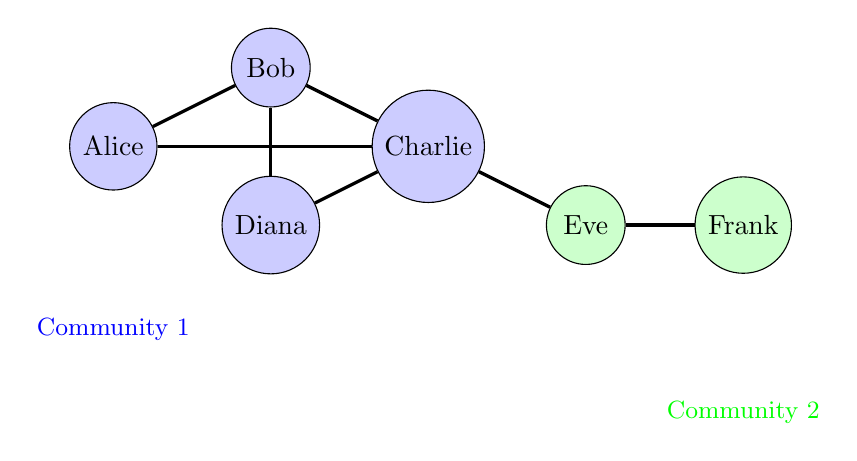
\begin{tikzpicture}[scale=1.0, every node/.style={scale=1.0}]
      % Nodes
      \node[draw, circle, minimum size=1cm, fill=blue!20] (alice) at (0, 2) {Alice};
      \node[draw, circle, minimum size=1cm, fill=blue!20] (bob) at (2, 3) {Bob};
      \node[draw, circle, minimum size=1cm, fill=blue!20] (charlie) at (4, 2) {Charlie};
      \node[draw, circle, minimum size=1cm, fill=blue!20] (diana) at (2, 1) {Diana};
      \node[draw, circle, minimum size=1cm, fill=green!20] (eve) at (6, 1) {Eve};
      \node[draw, circle, minimum size=1cm, fill=green!20] (frank) at (8, 1) {Frank};

      % Edges
      \draw[-, very thick] (alice) -- (bob);
      \draw[-, very thick] (alice) -- (charlie);
      \draw[-, very thick] (bob) -- (charlie);
      \draw[-, very thick] (bob) -- (diana);
      \draw[-, very thick] (charlie) -- (diana);
      \draw[-, very thick] (charlie) -- (eve);
      \draw[-, very thick] (eve) -- (frank);

      % Community labels
      \node[below=1.5cm of alice, font=\small, blue] {Community 1};
      \node[below=1.5cm of frank, font=\small, green] {Community 2};
    \end{tikzpicture}
  \end{center}

  \vspace{0.3cm}
  \textbf{Graph Metrics:}
  \begin{itemize}
    \item Alice to Frank: 4 degrees of separation (Alice $\to$ Charlie $\to$ Eve $\to$ Frank)
    \item Bob has highest clustering coefficient (friends are connected)
    \item Two communities visible
  \end{itemize}
\end{frame}

\begin{frame}[fragile]{Implementation: Social Network}
\begin{lstlisting}[language=Python, basicstyle=\tiny\ttfamily]
from collections import defaultdict, deque

class SocialNetwork:
    def __init__(self, directed=False):
        self.users = {}  # user_id -> User object
        self.graph = defaultdict(set)  # adjacency list
        self.directed = directed

    def add_connection(self, user1_id, user2_id):
        """Add friendship/follow relationship."""
        self.graph[user1_id].add(user2_id)
        if not self.directed:
            self.graph[user2_id].add(user1_id)

    def degrees_of_separation(self, user1_id, user2_id):
        """Find shortest path using BFS."""
        if user1_id == user2_id:
            return (0, [user1_id])

        visited = {user1_id}
        queue = deque([(user1_id, [user1_id])])

        while queue:
            current_id, path = queue.popleft()
            for friend_id in self.graph[current_id]:
                if friend_id == user2_id:
                    return (len(path), path + [friend_id])
                if friend_id not in visited:
                    visited.add(friend_id)
                    queue.append((friend_id, path + [friend_id]))

        return (-1, [])  # No path
\end{lstlisting}
\end{frame}

\begin{frame}[fragile]{Friend Suggestions Algorithm}
\begin{lstlisting}[language=Python, basicstyle=\tiny\ttfamily]
def suggest_friends(self, user_id, max_suggestions=5):
    """Suggest friends based on mutual connections."""
    current_friends = self.graph[user_id]
    mutual_counts = defaultdict(int)

    # Count mutual friends for non-friends
    for friend_id in current_friends:
        for friend_of_friend_id in self.graph[friend_id]:
            if (friend_of_friend_id != user_id and
                friend_of_friend_id not in current_friends):
                mutual_counts[friend_of_friend_id] += 1

    # Sort by mutual friend count
    suggestions = sorted(
        mutual_counts.items(),
        key=lambda x: x[1],
        reverse=True
    )[:max_suggestions]

    return [(self.users[uid], count) for uid, count in suggestions]
\end{lstlisting}

\vspace{0.2cm}
\textbf{Example:} Alice is friends with Bob and Charlie. Bob and Charlie are both friends with Diana. $\to$ Suggest Diana to Alice (2 mutual friends).
\end{frame}

\begin{frame}{Influence Metrics: PageRank}
  \begin{columns}
    \begin{column}{0.5\textwidth}
      \textbf{PageRank Algorithm:}
      \begin{itemize}
        \item Iterative computation
        \item User's influence = sum of friends' influence / their friend count
        \item Damping factor (0.85)
        \item Converges after iterations
      \end{itemize}

      \vspace{0.3cm}
      \textbf{Formula:}
      \[
      PR(u) = \frac{1-d}{N} + d \sum_{v \in \text{in}(u)} \frac{PR(v)}{|\text{out}(v)|}
      \]

      \small where $d=0.85$, $N$ = number of users
    \end{column}

    \begin{column}{0.5\textwidth}
      \textbf{Clustering Coefficient:}

      Measures how connected a user's friends are to each other.

      \[
      C(u) = \frac{\text{actual connections}}{\text{possible connections}}
      \]

      \vspace{0.3cm}
      \textbf{Interpretation:}
      \begin{itemize}
        \item $C = 1$: All friends know each other (tight community)
        \item $C = 0$: No friends know each other (bridge user)
        \item High clustering $\to$ local community
      \end{itemize}
    \end{column}
  \end{columns}
\end{frame}

\begin{frame}{Community Detection}
  \begin{columns}
    \begin{column}{0.5\textwidth}
      \textbf{Algorithm: Connected Components}
      \begin{enumerate}
        \item Start DFS from unvisited user
        \item Mark all reachable users as one community
        \item Repeat until all users visited
      \end{enumerate}

      \vspace{0.3cm}
      \textbf{Complexity:}
      \begin{itemize}
        \item Time: $O(V + E)$
        \item Space: $O(V)$
      \end{itemize}
    \end{column}

    \begin{column}{0.5\textwidth}
      \textbf{Advanced Methods:}
      \begin{itemize}
        \item Girvan-Newman (edge betweenness)
        \item Louvain method (modularity optimization)
        \item Label propagation
      \end{itemize}

      \vspace{0.3cm}
      \textbf{Applications:}
      \begin{itemize}
        \item Recommend groups
        \item Targeted advertising
        \item Influence propagation
        \item Network analysis
      \end{itemize}
    \end{column}
  \end{columns}
\end{frame}

% Autocomplete Engine
\section{Autocomplete Engine}

\begin{frame}{Project 4: Autocomplete Engine}
  \begin{columns}
    \begin{column}{0.5\textwidth}
      \textbf{Project Requirements:}
      \begin{itemize}
        \item Insert words with frequencies
        \item Search for words by prefix
        \item Suggest top-k completions
        \item Dynamic updates
        \item Handle large dictionaries
      \end{itemize}
    \end{column}

    \begin{column}{0.5\textwidth}
      \textbf{Core Data Structure:}
      \begin{itemize}
        \item \textbf{Trie} (prefix tree)
        \item Frequency tracking at nodes
        \item Priority queue for top-k
      \end{itemize}

      \vspace{0.3cm}
      \textbf{Complexity:}
      \begin{itemize}
        \item Insert: $O(m)$ where $m$ = word length
        \item Search: $O(m)$
        \item Autocomplete: $O(m + n)$ where $n$ = results
      \end{itemize}
    \end{column}
  \end{columns}
\end{frame}

\begin{frame}{Trie Structure for Autocomplete}
  \begin{center}
    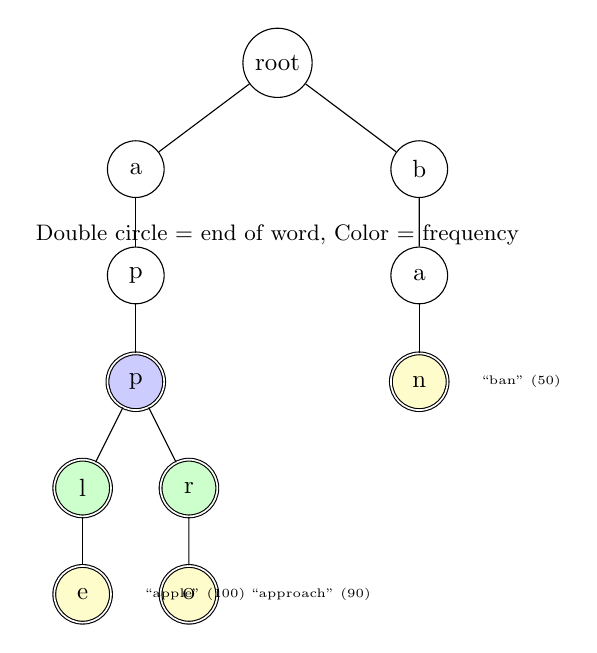
\begin{tikzpicture}[scale=0.9, every node/.style={scale=0.9},
      level 1/.style={sibling distance=40mm},
      level 2/.style={sibling distance=20mm},
      level 3/.style={sibling distance=15mm}]

      % Root
      \node[circle, draw, minimum size=0.8cm] (root) {root}
        child { node[circle, draw, minimum size=0.8cm] {a}
          child { node[circle, draw, minimum size=0.8cm] {p}
            child { node[circle, draw, double, minimum size=0.8cm, fill=blue!20] {p}
              child { node[circle, draw, double, minimum size=0.8cm, fill=green!20] {l}
                child { node[circle, draw, double, minimum size=0.8cm, fill=yellow!20] (apple) {e}
                  edge from parent node[left, font=\tiny] {}
                }
                edge from parent node[left, font=\tiny] {}
              }
              child { node[circle, draw, double, minimum size=0.8cm, fill=green!20] {r}
                child { node[circle, draw, double, minimum size=0.8cm, fill=yellow!20] (approach) {o}
                  edge from parent node[right, font=\tiny] {}
                }
                edge from parent node[right, font=\tiny] {}
              }
              edge from parent node[left, font=\tiny] {}
            }
            edge from parent node[left, font=\tiny] {}
          }
          edge from parent node[left, font=\tiny] {}
        }
        child { node[circle, draw, minimum size=0.8cm] {b}
          child { node[circle, draw, minimum size=0.8cm] {a}
            child { node[circle, draw, double, minimum size=0.8cm, fill=yellow!20] (ban) {n}
              edge from parent node[left, font=\tiny] {}
            }
            edge from parent node[right, font=\tiny] {}
          }
          edge from parent node[right, font=\tiny] {}
        };

      % Word annotations
      \node[right=0.3cm of apple, font=\tiny] {``apple'' (100)};
      \node[right=0.3cm of approach, font=\tiny] {``approach'' (90)};
      \node[right=0.3cm of ban, font=\tiny] {``ban'' (50)};

      % Legend
      \node[below=1.5cm of root, font=\small] {Double circle = end of word, Color = frequency};
    \end{tikzpicture}
  \end{center}

  \begin{itemize}
    \item Each path from root to double-circled node = one word
    \item Frequency stored at terminal nodes
    \item Prefix "app" $\to$ finds "apple" and "approach"
  \end{itemize}
\end{frame}

\begin{frame}[fragile]{Implementation: Trie Node and Insert}
\begin{lstlisting}[language=Python, basicstyle=\tiny\ttfamily]
class TrieNode:
    def __init__(self):
        self.children = {}  # char -> TrieNode
        self.is_end_of_word = False
        self.frequency = 0
        self.word = None

class AutocompleteEngine:
    def __init__(self):
        self.root = TrieNode()

    def insert(self, word: str, frequency: int = 1):
        """Insert word with frequency."""
        node = self.root
        for char in word.lower():
            if char not in node.children:
                node.children[char] = TrieNode()
            node = node.children[char]

        node.is_end_of_word = True
        node.word = word
        node.frequency += frequency

    def _find_node(self, prefix: str):
        """Find node corresponding to prefix."""
        node = self.root
        for char in prefix:
            if char not in node.children:
                return None
            node = node.children[char]
        return node
\end{lstlisting}
\end{frame}

\begin{frame}[fragile]{Autocomplete Algorithm}
\begin{lstlisting}[language=Python, basicstyle=\tiny\ttfamily]
def autocomplete(self, prefix: str, max_suggestions: int = 10):
    """Get autocomplete suggestions for prefix."""
    prefix = prefix.lower()
    node = self._find_node(prefix)

    if node is None:
        return []

    # Collect all words with this prefix
    suggestions = []
    self._collect_words(node, suggestions)

    # Sort by frequency and return top suggestions
    suggestions.sort(key=lambda x: x[1], reverse=True)
    return suggestions[:max_suggestions]

def _collect_words(self, node, suggestions):
    """Recursively collect all words from node."""
    if node.is_end_of_word:
        suggestions.append((node.word, node.frequency))

    for child in node.children.values():
        self._collect_words(child, suggestions)
\end{lstlisting}

\vspace{0.2cm}
\textbf{Example:} For prefix "app", collect all descendants: "apple" (100), "application" (80), "approach" (90). Sort by frequency and return top 10.
\end{frame}

\begin{frame}{Autocomplete: Advanced Features}
  \begin{columns}
    \begin{column}{0.5\textwidth}
      \textbf{Optimizations:}
      \begin{itemize}
        \item Min-heap for top-k (avoid sorting all)
        \item Store top-k at each node (cache)
        \item Compressed tries (radix tree)
        \item Limit recursion depth
      \end{itemize}

      \vspace{0.3cm}
      \textbf{Personalization:}
      \begin{itemize}
        \item User-specific frequency
        \item Recent searches
        \item Context-aware suggestions
        \item Location-based
      \end{itemize}
    \end{column}

    \begin{column}{0.5\textwidth}
      \textbf{Fuzzy Matching:}
      \begin{itemize}
        \item Allow typos (edit distance)
        \item Suggest corrections
        \item Phonetic matching
      \end{itemize}

      \vspace{0.3cm}
      \textbf{Real-World Applications:}
      \begin{itemize}
        \item Search engines (Google, Bing)
        \item Code editors (IDEs)
        \item Mobile keyboards
        \item E-commerce search
        \item Command-line interfaces
      \end{itemize}
    \end{column}
  \end{columns}
\end{frame}

% Memory Allocator Simulator
\section{Memory Allocator Simulator}

\begin{frame}{Project 5: Memory Allocator Simulator}
  \begin{columns}
    \begin{column}{0.5\textwidth}
      \textbf{Project Requirements:}
      \begin{itemize}
        \item Allocate memory blocks
        \item Free allocated blocks
        \item Coalesce adjacent free blocks
        \item Handle fragmentation
        \item Track usage statistics
        \item Multiple allocation strategies
      \end{itemize}
    \end{column}

    \begin{column}{0.5\textwidth}
      \textbf{Core Data Structure:}
      \begin{itemize}
        \item \textbf{Free list} (linked list)
        \item Hash table for allocated blocks
        \item Doubly-linked for coalescing
      \end{itemize}

      \vspace{0.3cm}
      \textbf{Strategies:}
      \begin{itemize}
        \item First-fit: $O(n)$
        \item Best-fit: $O(n)$
        \item Worst-fit: $O(n)$
      \end{itemize}
    \end{column}
  \end{columns}
\end{frame}

\begin{frame}{Memory Layout Visualization}
  \begin{center}
    \textbf{Memory Map (1000 bytes total):}

    \vspace{0.3cm}
    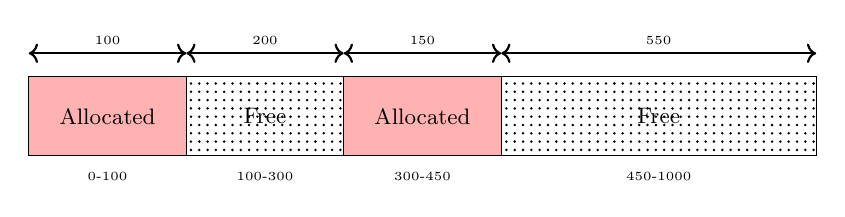
\begin{tikzpicture}[scale=1.0, every node/.style={scale=0.9}]
      % Memory blocks
      \draw[fill=red!30] (0, 0) rectangle (2, 1);
      \node at (1, 0.5) {\small Allocated};
      \node[below=0.1cm of {(1, 0)}, font=\tiny] {0-100};

      \draw[fill=green!20, pattern=dots] (2, 0) rectangle (4, 1);
      \node at (3, 0.5) {\small Free};
      \node[below=0.1cm of {(3, 0)}, font=\tiny] {100-300};

      \draw[fill=red!30] (4, 0) rectangle (6, 1);
      \node at (5, 0.5) {\small Allocated};
      \node[below=0.1cm of {(5, 0)}, font=\tiny] {300-450};

      \draw[fill=green!20, pattern=dots] (6, 0) rectangle (10, 1);
      \node at (8, 0.5) {\small Free};
      \node[below=0.1cm of {(8, 0)}, font=\tiny] {450-1000};

      % Arrows showing sizes
      \draw[<->, thick] (0, 1.3) -- (2, 1.3) node[midway, above, font=\tiny] {100};
      \draw[<->, thick] (2, 1.3) -- (4, 1.3) node[midway, above, font=\tiny] {200};
      \draw[<->, thick] (4, 1.3) -- (6, 1.3) node[midway, above, font=\tiny] {150};
      \draw[<->, thick] (6, 1.3) -- (10, 1.3) node[midway, above, font=\tiny] {550};
    \end{tikzpicture}
  \end{center}

  \vspace{0.3cm}
  \textbf{Allocation Request (50 bytes):}
  \begin{itemize}
    \item \textbf{First-fit}: Use free block at 100-300 (first available)
    \item \textbf{Best-fit}: Use free block at 100-300 (smallest that fits)
    \item \textbf{Worst-fit}: Use free block at 450-1000 (largest)
  \end{itemize}
\end{frame}

\begin{frame}[fragile]{Implementation: Memory Block}
\begin{lstlisting}[language=Python, basicstyle=\tiny\ttfamily]
class MemoryBlock:
    def __init__(self, start: int, size: int, is_free: bool = True):
        self.start = start
        self.size = size
        self.is_free = is_free
        self.next = None  # Next block in list
        self.prev = None  # Previous block in list

    @property
    def end(self):
        return self.start + self.size

class MemoryAllocator:
    def __init__(self, total_size: int, strategy):
        self.total_size = total_size
        self.strategy = strategy
        self.head = MemoryBlock(0, total_size, is_free=True)
        self.allocated_blocks = {}  # address -> block

    def malloc(self, size: int):
        """Allocate memory block."""
        block = self._find_free_block(size)
        if block is None:
            return None  # Allocation failed
        if block.size > size:
            self._split_block(block, size)
        block.is_free = False
        self.allocated_blocks[block.start] = block
        return block.start
\end{lstlisting}
\end{frame}

\begin{frame}[fragile]{Coalescing Adjacent Free Blocks}
\begin{lstlisting}[language=Python, basicstyle=\tiny\ttfamily]
def free(self, address: int):
    """Free allocated block."""
    if address not in self.allocated_blocks:
        return False

    block = self.allocated_blocks[address]
    del self.allocated_blocks[address]
    block.is_free = True

    # Coalesce with adjacent free blocks
    self._coalesce(block)
    return True

def _coalesce(self, block):
    """Merge adjacent free blocks."""
    # Coalesce with next block
    if block.next and block.next.is_free:
        block.size += block.next.size
        block.next = block.next.next
        if block.next:
            block.next.prev = block

    # Coalesce with previous block
    if block.prev and block.prev.is_free:
        block.prev.size += block.size
        block.prev.next = block.next
        if block.next:
            block.next.prev = block.prev
\end{lstlisting}
\end{frame}

\begin{frame}{Coalescing Example}
  \begin{center}
    \textbf{Before Coalescing:}

    \vspace{0.2cm}
    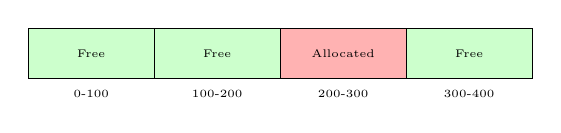
\begin{tikzpicture}[scale=0.8, every node/.style={scale=0.8}]
      \draw[fill=green!20] (0, 0) rectangle (2, 0.8);
      \node at (1, 0.4) {\tiny Free};
      \node[below=0.05cm of {(1, 0)}, font=\tiny] {0-100};

      \draw[fill=green!20] (2, 0) rectangle (4, 0.8);
      \node at (3, 0.4) {\tiny Free};
      \node[below=0.05cm of {(3, 0)}, font=\tiny] {100-200};

      \draw[fill=red!30] (4, 0) rectangle (6, 0.8);
      \node at (5, 0.4) {\tiny Allocated};
      \node[below=0.05cm of {(5, 0)}, font=\tiny] {200-300};

      \draw[fill=green!20] (6, 0) rectangle (8, 0.8);
      \node at (7, 0.4) {\tiny Free};
      \node[below=0.05cm of {(7, 0)}, font=\tiny] {300-400};
    \end{tikzpicture}

    \vspace{0.5cm}
    \textbf{After Coalescing:}

    \vspace{0.2cm}
    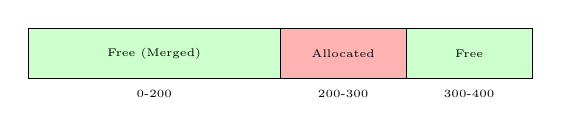
\begin{tikzpicture}[scale=0.8, every node/.style={scale=0.8}]
      \draw[fill=green!20] (0, 0) rectangle (4, 0.8);
      \node at (2, 0.4) {\tiny Free (Merged)};
      \node[below=0.05cm of {(2, 0)}, font=\tiny] {0-200};

      \draw[fill=red!30] (4, 0) rectangle (6, 0.8);
      \node at (5, 0.4) {\tiny Allocated};
      \node[below=0.05cm of {(5, 0)}, font=\tiny] {200-300};

      \draw[fill=green!20] (6, 0) rectangle (8, 0.8);
      \node at (7, 0.4) {\tiny Free};
      \node[below=0.05cm of {(7, 0)}, font=\tiny] {300-400};
    \end{tikzpicture}
  \end{center}

  \vspace{0.3cm}
  \textbf{Benefits:}
  \begin{itemize}
    \item Reduces fragmentation
    \item Creates larger free blocks
    \item Improves allocation success rate
    \item Essential for long-running systems
  \end{itemize}
\end{frame}

\begin{frame}{Allocation Strategy Comparison}
  \begin{table}
    \centering
    \small
    \begin{tabular}{lccc}
      \hline
      \textbf{Strategy} & \textbf{Speed} & \textbf{Fragmentation} & \textbf{Use Case} \\
      \hline
      First-Fit & Fast & Moderate & General purpose \\
      Best-Fit & Slow & Low & Memory constrained \\
      Worst-Fit & Slow & High & Large allocations \\
      \hline
    \end{tabular}
  \end{table}

  \vspace{0.3cm}
  \textbf{Trade-offs:}
  \begin{itemize}
    \item \textbf{First-Fit}: Fast but may create small unusable fragments at start
    \item \textbf{Best-Fit}: Minimizes wasted space but creates tiny fragments
    \item \textbf{Worst-Fit}: Keeps large blocks available but wastes space
  \end{itemize}

  \vspace{0.3cm}
  \textbf{Real-World:} Most allocators use variants of first-fit with segregated free lists for different size classes (e.g., jemalloc, tcmalloc).
\end{frame}

% Project Structuring and Testing
\section{Project Structuring and Testing}

\begin{frame}{Project Structure Best Practices}
  \begin{columns}
    \begin{column}{0.5\textwidth}
      \textbf{Directory Layout:}
      \begin{itemize}
        \item \texttt{src/} - Source code
        \begin{itemize}
          \item \texttt{data\_structures/}
          \item \texttt{algorithms/}
          \item \texttt{utils/}
        \end{itemize}
        \item \texttt{tests/} - Test files
        \item \texttt{docs/} - Documentation
        \item \texttt{requirements.txt}
        \item \texttt{README.md}
        \item \texttt{setup.py}
      \end{itemize}
    \end{column}

    \begin{column}{0.5\textwidth}
      \textbf{Principles:}
      \begin{itemize}
        \item Separate concerns
        \item One class per file (large projects)
        \item Clear naming conventions
        \item Package initialization files
        \item Version control (git)
      \end{itemize}

      \vspace{0.3cm}
      \textbf{Documentation:}
      \begin{itemize}
        \item Docstrings for all public APIs
        \item README with usage examples
        \item API reference
        \item Architecture diagrams
      \end{itemize}
    \end{column}
  \end{columns}
\end{frame}

\begin{frame}{Testing Strategies}
  \begin{columns}
    \begin{column}{0.5\textwidth}
      \textbf{Unit Tests:}
      \begin{itemize}
        \item Test individual methods
        \item Isolate dependencies
        \item Fast execution
        \item High coverage
      \end{itemize}

      \vspace{0.2cm}
      \textbf{Integration Tests:}
      \begin{itemize}
        \item Test component interaction
        \item End-to-end scenarios
        \item Realistic workloads
      \end{itemize}

      \vspace{0.2cm}
      \textbf{Edge Cases:}
      \begin{itemize}
        \item Empty inputs
        \item Maximum sizes
        \item Invalid inputs
        \item Boundary conditions
      \end{itemize}
    \end{column}

    \begin{column}{0.5\textwidth}
      \textbf{Performance Tests:}
      \begin{itemize}
        \item Benchmark operations
        \item Verify complexity
        \item Regression testing
        \item Memory usage
      \end{itemize}

      \vspace{0.2cm}
      \textbf{Property-Based Testing:}
      \begin{itemize}
        \item Test invariants
        \item Generate random inputs
        \item Find edge cases automatically
        \item Use hypothesis library
      \end{itemize}

      \vspace{0.2cm}
      \textbf{Tools:}
      \begin{itemize}
        \item \texttt{unittest}, \texttt{pytest}
        \item \texttt{coverage.py}
        \item CI/CD (GitHub Actions)
      \end{itemize}
    \end{column}
  \end{columns}
\end{frame}

\begin{frame}[fragile]{Testing Example: Text Editor}
\begin{lstlisting}[language=Python, basicstyle=\tiny\ttfamily]
import unittest

class TestTextEditor(unittest.TestCase):
    def setUp(self):
        self.editor = TextEditor()

    def test_insert_at_beginning(self):
        self.editor.insert(0, "Hello")
        self.assertEqual(self.editor.get_text(), "Hello")

    def test_undo_redo_sequence(self):
        self.editor.insert(0, "A")
        self.editor.insert(1, "B")
        self.editor.undo()
        self.assertEqual(self.editor.get_text(), "A")
        self.editor.redo()
        self.assertEqual(self.editor.get_text(), "AB")

    def test_redo_cleared_on_new_operation(self):
        self.editor.insert(0, "Test")
        self.editor.undo()
        self.editor.insert(0, "New")
        self.assertFalse(self.editor.can_redo())

    def test_large_text_operations(self):
        large_text = "x" * 10000
        self.editor.insert(0, large_text)
        self.assertEqual(len(self.editor.get_text()), 10000)
\end{lstlisting}
\end{frame}

\begin{frame}{Code Quality and Best Practices}
  \begin{columns}
    \begin{column}{0.5\textwidth}
      \textbf{Code Style:}
      \begin{itemize}
        \item Follow PEP 8 (Python)
        \item Consistent naming
        \item Clear variable names
        \item Avoid magic numbers
        \item Type hints
      \end{itemize}

      \vspace{0.2cm}
      \textbf{Error Handling:}
      \begin{itemize}
        \item Validate inputs
        \item Raise appropriate exceptions
        \item Document error conditions
        \item Fail fast
      \end{itemize}
    \end{column}

    \begin{column}{0.5\textwidth}
      \textbf{Performance:}
      \begin{itemize}
        \item Profile before optimizing
        \item Document complexity
        \item Avoid premature optimization
        \item Test performance
      \end{itemize}

      \vspace{0.2cm}
      \textbf{Maintenance:}
      \begin{itemize}
        \item Regular refactoring
        \item Keep functions small
        \item Single responsibility principle
        \item Version control commits
        \item Code reviews
      \end{itemize}
    \end{column}
  \end{columns}
\end{frame}

% Summary
\section{Summary}

\begin{frame}{Projects Summary}
  \begin{table}
    \centering
    \small
    \begin{tabular}{lcc}
      \hline
      \textbf{Project} & \textbf{Core Structure} & \textbf{Key Algorithm} \\
      \hline
      Text Editor & Stack & Command pattern \\
      DB Index & B-Tree & Split/merge \\
      Social Network & Graph & BFS, PageRank \\
      Autocomplete & Trie & Prefix traversal \\
      Memory Allocator & Free List & Coalescing \\
      \hline
    \end{tabular}
  \end{table}

  \vspace{0.3cm}
  \textbf{Common Themes:}
  \begin{itemize}
    \item Choose data structure based on operations
    \item Combine multiple structures when needed
    \item Test thoroughly (unit, integration, edge cases)
    \item Measure and document performance
    \item Maintain clean, readable code
  \end{itemize}
\end{frame}

\begin{frame}{Key Takeaways}
  \begin{enumerate}
    \item \textbf{Data Structures Enable Solutions}
    \begin{itemize}
      \item Stacks enable undo/redo naturally
      \item B-Trees excel at disk-based sorted data
      \item Graphs model relationships and networks
      \item Tries optimize prefix-based search
      \item Free lists manage dynamic memory
    \end{itemize}

    \vspace{0.2cm}
    \item \textbf{Design Matters}
    \begin{itemize}
      \item Understand requirements before choosing structures
      \item Consider time/space trade-offs
      \item Plan for scalability and edge cases
    \end{itemize}

    \vspace{0.2cm}
    \item \textbf{Testing is Essential}
    \begin{itemize}
      \item Comprehensive tests catch bugs early
      \item Property-based tests find unexpected issues
      \item Performance tests verify complexity
    \end{itemize}
  \end{enumerate}
\end{frame}

\begin{frame}{Building Your Portfolio}
  \textbf{Next Steps:}
  \begin{enumerate}
    \item \textbf{Implement These Projects}
    \begin{itemize}
      \item Start with text editor (simplest)
      \item Work up to memory allocator (most complex)
      \item Add your own features and extensions
    \end{itemize}

    \vspace{0.2cm}
    \item \textbf{Extend and Experiment}
    \begin{itemize}
      \item Add GUI to text editor
      \item Implement concurrent B-Tree
      \item Add recommendation system to social network
      \item Build fuzzy matching for autocomplete
      \item Compare allocation strategies empirically
    \end{itemize}

    \vspace{0.2cm}
    \item \textbf{Document and Share}
    \begin{itemize}
      \item Write clear READMEs
      \item Create demonstrations
      \item Share on GitHub
      \item Discuss in interviews
    \end{itemize}
  \end{enumerate}
\end{frame}

\begin{frame}{Additional Project Ideas}
  \textbf{More Projects to Try:}
  \begin{itemize}
    \item \textbf{Task Scheduler}: Priority queue + heap for job scheduling
    \item \textbf{File System Simulator}: Tree + hash table for directories
    \item \textbf{LRU Cache}: Hash table + doubly-linked list
    \item \textbf{Spell Checker}: Trie + edit distance algorithm
    \item \textbf{Git-like Version Control}: DAG + hash table
    \item \textbf{JSON Parser}: Stack for nested structures
    \item \textbf{URL Shortener}: Hash table + base conversion
    \item \textbf{Rate Limiter}: Queue + sliding window
    \item \textbf{Expression Evaluator}: Stack + parsing
    \item \textbf{Prefix Sum Range Queries}: Segment tree or Fenwick tree
  \end{itemize}

  \vspace{0.3cm}
  \begin{block}{Remember}
    The best way to learn data structures is to use them to solve real problems!
  \end{block}
\end{frame}

\begin{frame}
  \begin{center}
    {\Huge Thank You!}

    \vspace{1cm}
    {\Large Questions?}

    \vspace{1cm}
    \textit{``The only way to learn a new programming language \\
    is by writing programs in it.'' -- Dennis Ritchie}

    \vspace{0.5cm}
    \small The same applies to data structures: \\
    learn by building projects!
  \end{center}
\end{frame}

\end{document}
